\section{Introduction}
\label{sec:introduction}

In modern data centers, the efficient utilization of resources is crucial for optimal performance and cost-effectiveness. One of the challenges faced by these systems is the presence of stranded memory, which refers to allocated but unused memory. As seen in Figure \ref{fig:Stranded_memory}, over 30\% of the memory in modern data-centers is stranded. This stranded memory often co-exists with overutilized CPUs, leading to an imbalance in resource utilization. Prior works \cite{Infiniswap, Fastswap, Hermit, AdvancesAndChallenges, Redy} have sought to address this issue by efficiently utilizing this stranded memory in various ways, such as exposing the remote memory pool as a swap device \cite{Infiniswap, Fastswap, Hermit}; utilizing stranded memory as dynamic cache \cite{Redy}. In this project, we specifally focus on utilizing the stranded memory to build a cache for images. We propose ImageHarbour, a system that aggregates stranded memory from multiple hosts into a single, large memory pool and exposes it as a shared image cache that can be accessed by all the servers in the cluster.

\begin{figure}[h]
    \centering
    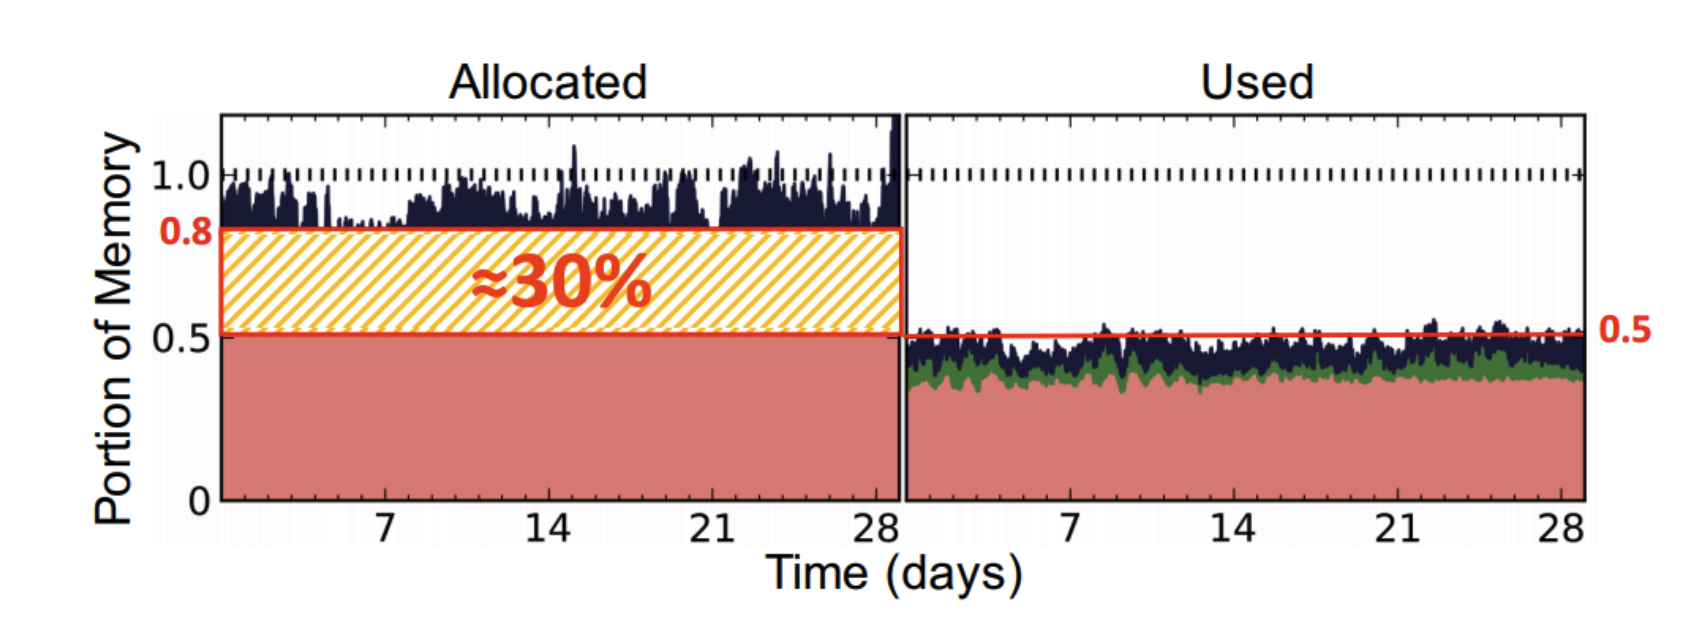
\includegraphics[width=0.45\textwidth]{Stranded_memory.png}
    \caption{Stranded memory in modern datacenters \cite{reiss2012heterogeneity}}
    \label{fig:Stranded_memory}
\end{figure}

ImageHarbour draws inspiration from two key concepts: stranded memory and efficient memory disaggregation. The notion of stranded memory is derived from the study by Reiss et al. \cite{reiss2012heterogeneity}, which highlights the presence of allocated but unused memory in Google's data centers. Their analysis reveals that while some nodes have high CPU utilization, their memory remains underutilized, resulting in stranded memory. The idea of efficient memory disaggregation is motivated by Infiniswap\cite{Infiniswap}, a remote memory paging system that leverages one-sided Remote Direct Memory Access (RDMA) operations to access memory on remote nodes without interrupting the CPU on the remote node.

RDMA is a high-performance networking technology that allows direct memory access from the memory of one computer to that of another without involving either computer's operating system \cite{kalia2016design}. Additionally, one-sided RDMA access does not interrupt the CPU on the remote memory node. This enables low-latency and high-bandwidth communication between nodes in a data center. By exploiting one-sided RDMA operations, ImageHarbour can efficiently access memory on remote nodes with minimal overhead, achieving latencies in the sub-microsecond range. 

Our key observation is that retrieving an image using one-sided RDMA operations provides significantly better latencies (sub-microsecond) while not consuming CPU cycles on the memory server, than conventional methods to retrieve images. For example, traditional disk-based storage systems have latencies around 5-10 milliseconds for a 4KB read operation \cite{yang2014don}, while retrieving Docker images over the internet can take seconds to minutes, depending on the image size and network conditions \cite{harter2016slacker}.

ImageHarbour leverages these observations to create a distributed image caching system that can significantly improve the performance of image-based workloads in data centers. By pooling together stranded memory from multiple hosts, ImageHarbour creates a large, unified memory pool that can be used to cache frequently accessed Docker images. ImageHarbour exposes an image server that intelligently manages the cache, decides which images to bring in, which images to evict, and serves metadata to the clients regarding the location of cached images within the memory pool.

Clients accessing the cached images through ImageHarbour experience significantly reduced latencies compared to traditional image retrieval methods. By serving images directly from memory using one-sided RDMA operations, ImageHarbour can achieve up to 9x lower latency compared to storing the image on the disk or using a local repository and upto 74x lower latency compared to downloading images over the internet.
